\section{Motivation}
\label {sec:motiv}
\subsection{Replicated Data Types in ECDS }
\begin{figure}[t]
        \centering
	\begin{subfigure}[b]{0.489\textwidth}
	\begin{lstlisting}
type Effect = String 
type State =  String 

read :: State -> (String,Maybe Effect)
read s = (s,Nothing)

write :: String -> ((),Maybe Effect)
write comment = ((),comment)

apply :: State -> Effect -> State 
apply s eff = in s ++ " - " ++ comment
	\end{lstlisting}
	\caption{A simple implementation}
	\label{subfig:comment_code}
	\end{subfigure}
	\hfill
	\begin{subfigure}[b]{0.475\textwidth}
	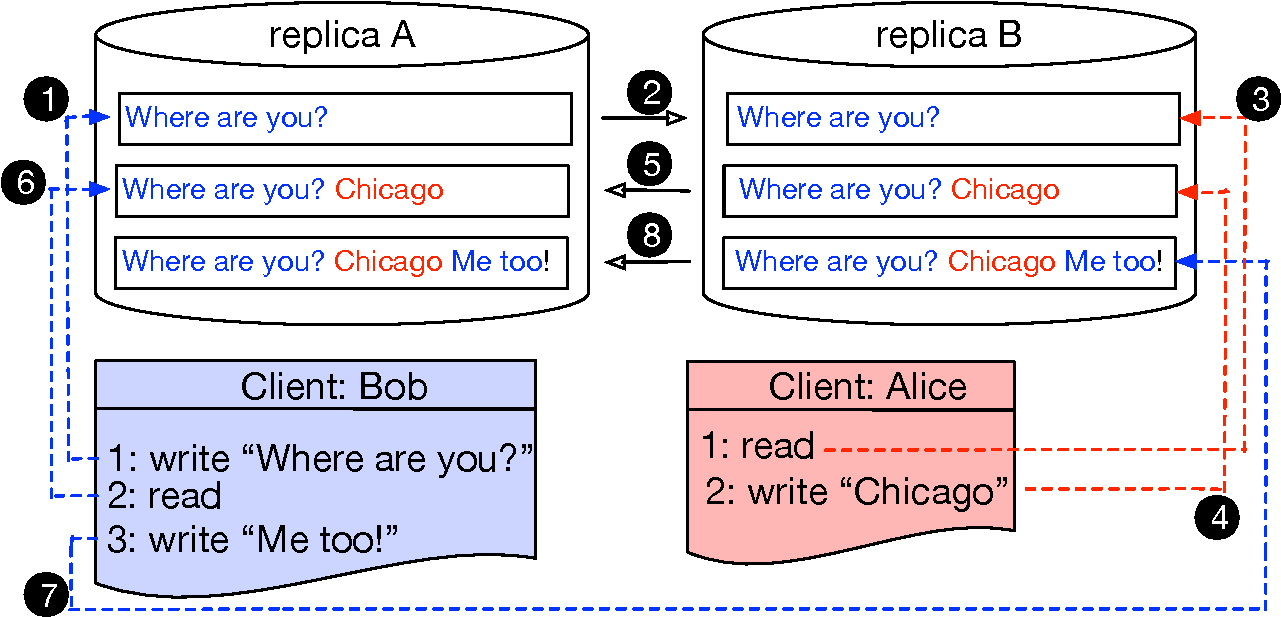
\includegraphics[scale=0.282]{Figures/comment_application.pdf}
	\caption{Example execution}
	\label{subfig:comment_example}
	\end{subfigure} 
\\ \hrulefill
\caption{A distributed application for comment section
management}
\label{fig:comment_app}
\end{figure}




%intro
To motivate our approach, consider a highly available (low
latency) application for managing comments on posts in 
a photo sharing web site.  Fig.~\ref{subfig:comment_code}
presents a simple Haskell implementation of such an application
cognizant of our system model.  
%impl

In this implementation, \effectC{} and \stateC{} strings are
respectively defined as the text of a single comment, and the
concatentation of all visible comments associated with a post.  A new
\effectC{} is generated every time a user wants to comment on a post
by calling the \writeC{} function, and a \readC{} call simply returns
the \stateC{} of the object at the serving replica.  The \applyC{}
function, returns the updated state of the replica, which is the
concatenation of the old state and the given effect.  For perspicuity,
we omit any conflict resolution strategy in the code; however,
developers (using timestamps, roll-backs, etc.) can design the
\applyC{} function to resolve conflicting concurrent updates as they
desire, consistent with application invariants.

%explaining the figure and how users interact with the system
An example of how users interact with this application is presented in
Fig.\ref{subfig:example_exec}, where Alice and Bob invoke operations
on an object (here, a photo of Alice in Chicago); the chronological
order of events is given in black circles.  At time \ding{182}, Bob
writes a comment, which is routed to replica \replO{1}, whose effect
is then propagated and delivered to replica \replO{2} at \ding{183};
while Alice's first read operation is routed to \ding{184}.  Alice and
Bob then keep talking, generating more read and write events, while
updates are propagated concurrently between the two replica.

%explain the anomaly possible in this setting
As mentioned before, lost updates, is a well-known, often undesirable,
behavior admitted by eventually consistent data stores (ECDS).  An
example of such anomaly can occur here if at time \ding{187}, Bob is
temporarily disconnected from both replicas in the figure, and his
read operation is routed to another replica \replO{3}, that has not
yet received any updates from \replO{1} or \replO{2}. Consequently,
Bob cannot see his first comment and would retry submitting it,
assuming it failed the first time it was sent.  This would result in
multiple copies of the message eventually being displayed on each
replica.


%
\subsection{Ad-hoc Anomaly Prevention}
One way to prevent the above anomaly is to tag each effect using a
unique identifier as mentioned in Sec.~\ref{sec:sys_model}. Using
these tags, replicas will be able to track all locally available
effects, and temporarily \emph{block} operations, until all the
preceding effects from the same session arrive at the replica. For
example, the replica \replO{3} that receives Bob's read in the above
undesired scenario, can simply postpone its execution until all prior
effects upon which this operation depends reach this replica..

In order to reduce the overhead of tracking dependencies per
operation, the above idea can be refined using another technique
called \emph{filtration}, which is based on separating the locally
available effects at each replica that have not yet been applied to
the state from those who have. In the above example each replica can
maintain a \emph{safe environment} for operations (e.g. using a
soft-state cache), that contains an effect only if it also contains
all the previous effects from the same session. This way, an operation
can proceed, when the effect of its  previous operation from the same
session is already applied to the state (which transitively yields the
presence of all dependencies).

We present a modified version of the running example in
Appendix~\ref{appendix:app}, updated to tolerate the lost-update
anomaly by implementing the blocking mechanism in the \readC{}
function and incorporating filtration in the \applyC{} function as
explained above. Unfortunately, these modifications require
fundamental and pervasive changes to the original code.  Additionally,
the changes are heavily tangled with application logic, complicating
reasoning, hampering correctness arguments, and sacrificing
composability and scalability.

%%SJ: I didn't follow this paragraph
%% Another major drawback of this approach arise in stores that do not
%% admit metadata queries (e.g. Cassandra)   is the \emph{lost
%%   histories}\cite{bolton} problem. To face this problem, for each new
%% session joining, the replicas must perforom a table alteration at the
%% data store level, to accomodate the data on the newly joined session.
%% This requires strong synchronization of replicas, degrading
%% application performance and availability.  Moreover, to make the
%% matter worse, new anomalies are constantly found in the systems after
%% the design phase, which require non-trivial, further polluting, ad-hoc
%% solutions that leave the existing implementation obsolete.





%
%--- What is our alternative approach
%
\subsection{Our Solution}
\tool is a runtime enforcement mechanism that allows developers to
define a consistency level for each operation \emph{a priori},
delegating the responsibility for ensuring that constraints defined by
this level are respected.  Our technique generalizes blocking and
filtration mechanisms, admits arbitrary user-defined dependency
relations for each operation, and maintains a consistent \emph{shim
  layer} on top of each ECDS replica.

\begin{wrapfigure}{i}{0.2\textwidth}
\centering
	\vspace{-10mm}
	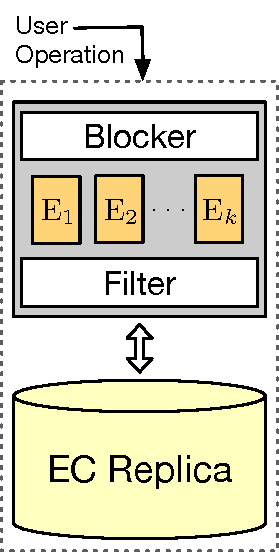
\includegraphics[scale=0.42]{Figures/outline.pdf}
	\label{fig:syncope_outline}
	\caption{\footnotesize \tool}
\label{fig:syncope_outline}
\vspace{-5mm}
\end{wrapfigure}



The \tool shim layer maintains multiple safe environments
({\footnotesize $E_1,E_2,...$}) by periodically (or on-demand) reading
from the underlying ECDS database, and adding effects to each
environment, only if its dependencies have already been added
(Fig.\ref{fig:syncope_outline}).  \tool realizes this idea
efficiently, using a simple tagging mechanism that represents effects
in an environment via a tag associated with that environment. Each
operation only witnesses effects from its associated environment, and
is blocked by the runtime system if the necessary dependencies are not
present.

%%%SJ: The second sentence should be expanded - what is a ``read''
%%% operation; what do you mean by ``synthesize''
Users can specify arbitrary consistency guarantees in a language that
is seeded with $\soO$ and $\visO$ relations.  Constraints on read
operations can be used to synthesize appropriate filtration and
blocking mechanisms.  For example, the following \emph{contract},
eliminates the possibilty of lost-update anomalies by establishing the
appropriate conditions under which an effect may be witnessed by the
current operation:
\begin{fmathpar}
\begin{array}{lllll}

\psi: & \forall a. &  \xrightarrow{\soZ} \hat{\eff} & \Rightarrow
& a
\xrightarrow {\visZ} \hat{\eff}  \\
\end{array}
\end{fmathpar}





















